%!TEX root = 0_document_de.tex
\section{Scope}
Deicing of a LiDAR sensor is necessary to provide a clear sight. The heat generated by a sensor itself is typically not sufficient for defrosting ice accumulated on the outer surface (see appendix A.1). Thats true in particular at low temperatures and high wind speeds resulting in a need for integrating an active heating element in the system. Finding the right heating layout can be a complex problem that is shaped by the requirement to maintain the optical quality during heating and to achieve a high heating performance in parallel. Which heating performance is required depends on use cases. For deicing the system must be designed in such a way that the available heating power is sufficient to heat up the surface temperature above \(0\dC\) for a specified range of ambient temperatures and wind speeds. Every design must be verified to meet this goal and the verification is usually achieved by a sophisticated simulation or experiment. The aim of this document is to ease the verification process by providing a description of the heat flow in a plane front cover with different heating layouts and finding a (semi-)analytical expression for the surface temperature. Only steady conditions and temperatures are considered. The model accuracy is demonstrated for the NEXT LiDAR sensor. In addition, a Matlab script based on finite element analysis is provided to solve the heat transfer problem for a 3-D model of the NEXT LiDAR front cover (see appendix A.3). 

In general, the surface temperature depends on the following influences:

\underline{Environmental influences}
\begin{itemize}
\item Ambient temperature \(T_{o}\)
\item Relative wind speed \(v\)
\item Precipitation on the surface
\end{itemize}

\underline{Design and control parameters}
\begin{itemize}
\item Heating power \(P\) or temperature of the heating wire/plate \(T_{hs}\)
\item Front cover design (thickness, distance between wires, ...)
\item Material (composition) of the front cover
\item Internal heat transfer from the LiDAR sensor electronics to the surface
\item Mounting position (in the car)
\end{itemize}

\begin{figure} [H]
	\centering
	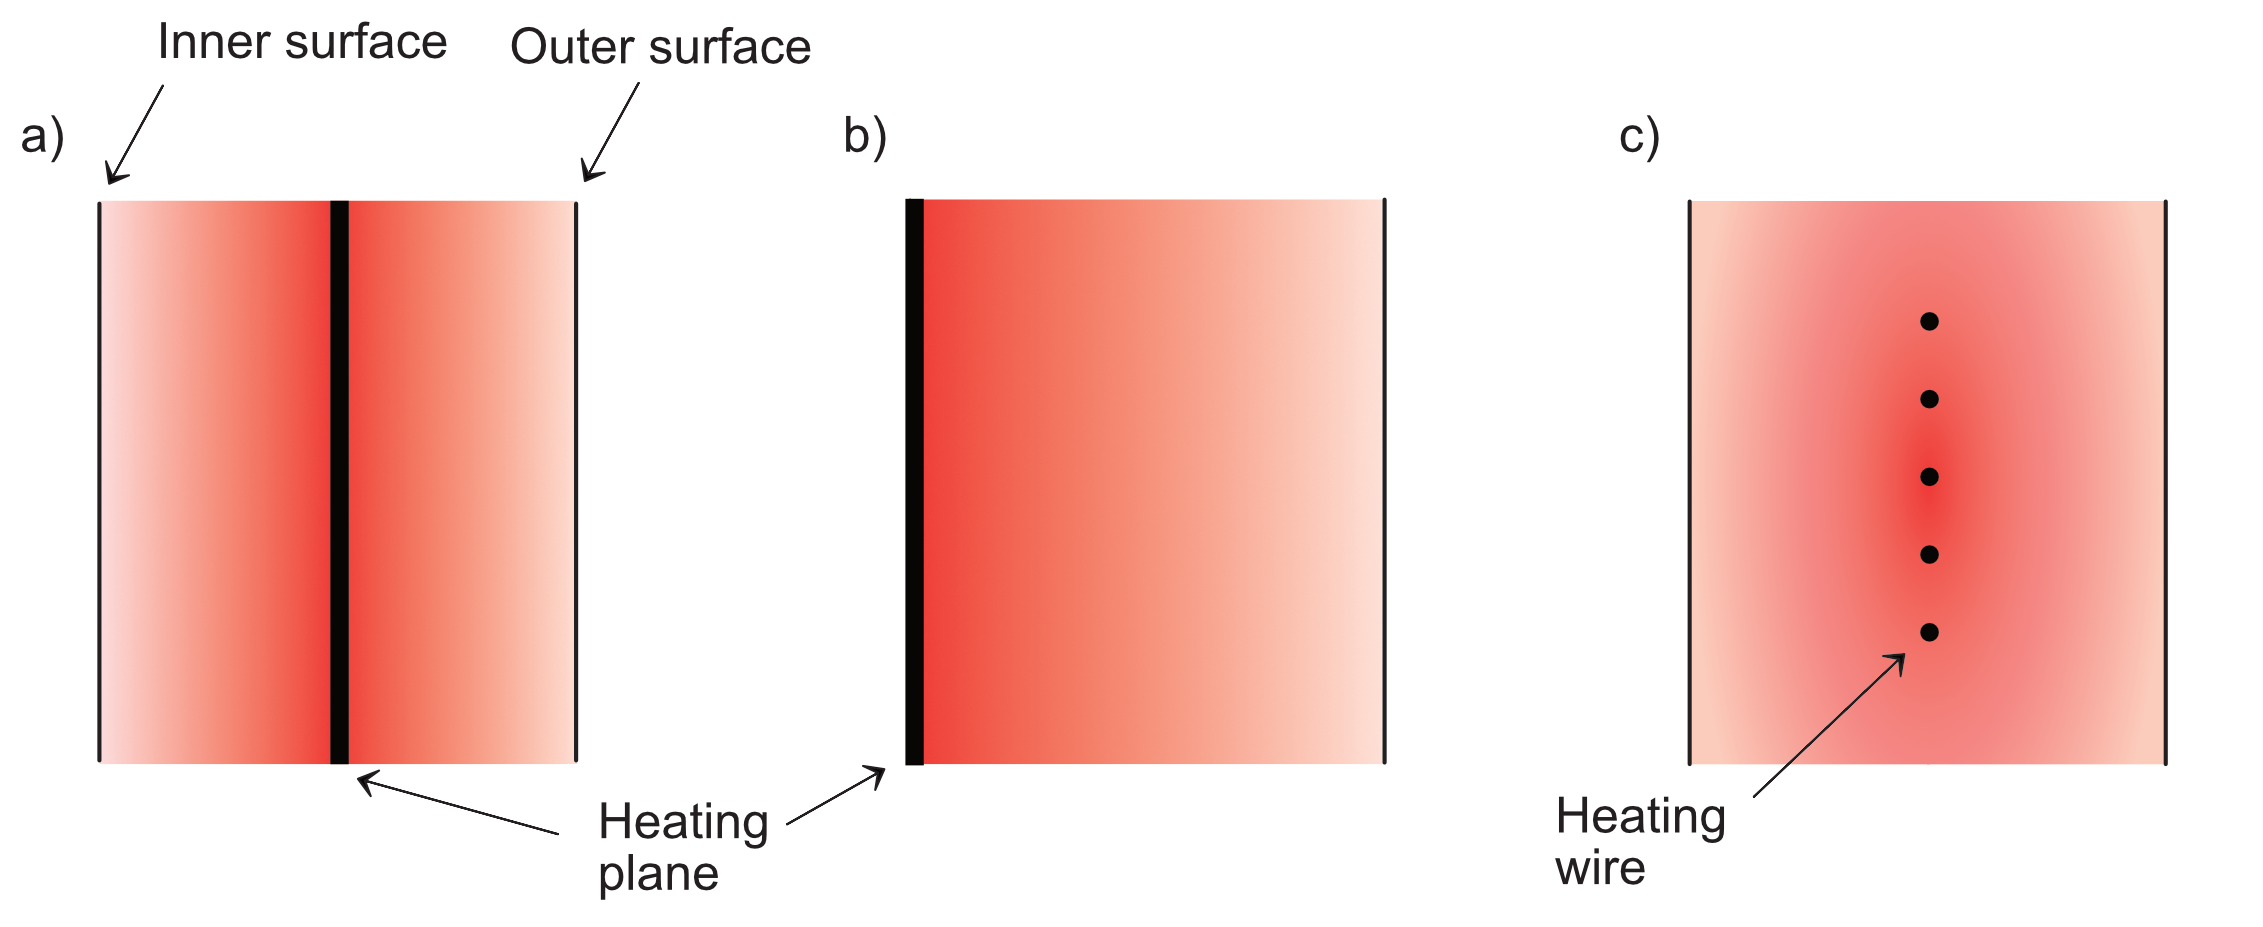
\includegraphics[scale=0.75]{Pictures/FrontCoverTypes.png}
	\caption[Heating Architectures]{Side view on three front covers with different heating architectures where a) a heating plate is buried in the mid plane b) a heating plate is attached to the inner surface and c) a row of equally spaced parallel heating wires are buried in the mid plane.}
	\label{fig:examples}
\end{figure}


\section{Generic Thermodynamic Model}
In this section, a generic analytical expression for the surface temperature of a (LiDAR) sensor is derived as a function of relative wind speed, ambient temperature and the heating power applied to the heating element. The expression can be applied to planar front covers in thermodynamic equilibrium. 

Many thermodynamic problems encountered in practice are two- or three-dimensional and involve rather complicated geometries for which no simple solutions exist. The front cover of the NEXT sensor shown in Fig. \ref{fig:1TB1Model} is such an example. One-dimensional geometries have exact solutions. Figures \ref{fig:examples}a and \ref{fig:examples}b show the sideview of two heating geometries of which simple analytical solutions can be derived. The geometry in Fig. \ref{fig:examples}c is a two-dimensional problem and requires a more elaborate calculation. Nonetheless, the solution is identical to the solution of the geometry in Fig. 1a when introducing a shape factor. This shape factor must be adjusted accordingly for more complex heating architectures such as the NEXT sensors front cover and can be found only numerically or experimentally. 

In the following, first the basic underlying thermodynamic expressions are introduced. Secondly, the surface temperature of the heating plate architecture shown in Fig. \ref{fig:examples}a is derived. Based on this solution, a general equation for more complex, planar geometries is dervied by introducing the shape factor.

\subsection{Thermodynamic Model}\label{chapter:basics}
Heat transfered per unit time, \(\dot Q\), through a wall of thickness \(d\) and area \(A\) depends on the temperature difference \(T_i - T_o\) between the inner side and the outer side of the wall:
\begin{equation}
\frac{\dot Q}{A} =  \frac{1}{R_{tot}}\cdot (T_i - T_o)
\end{equation}
with \(R_{tot}\) being the total thermal resistance of the wall. The heat is transfered by conduction through the material and by convection of air and radiation from inside to the wall and also from the wall to the outside. Heat transfered by radiation only need to be considered if the temperatures in the system are very high and the convection is weak (no wind). This situation does not apply for the NEXT sensor. 

\begin{figure} [H]
	\centering
	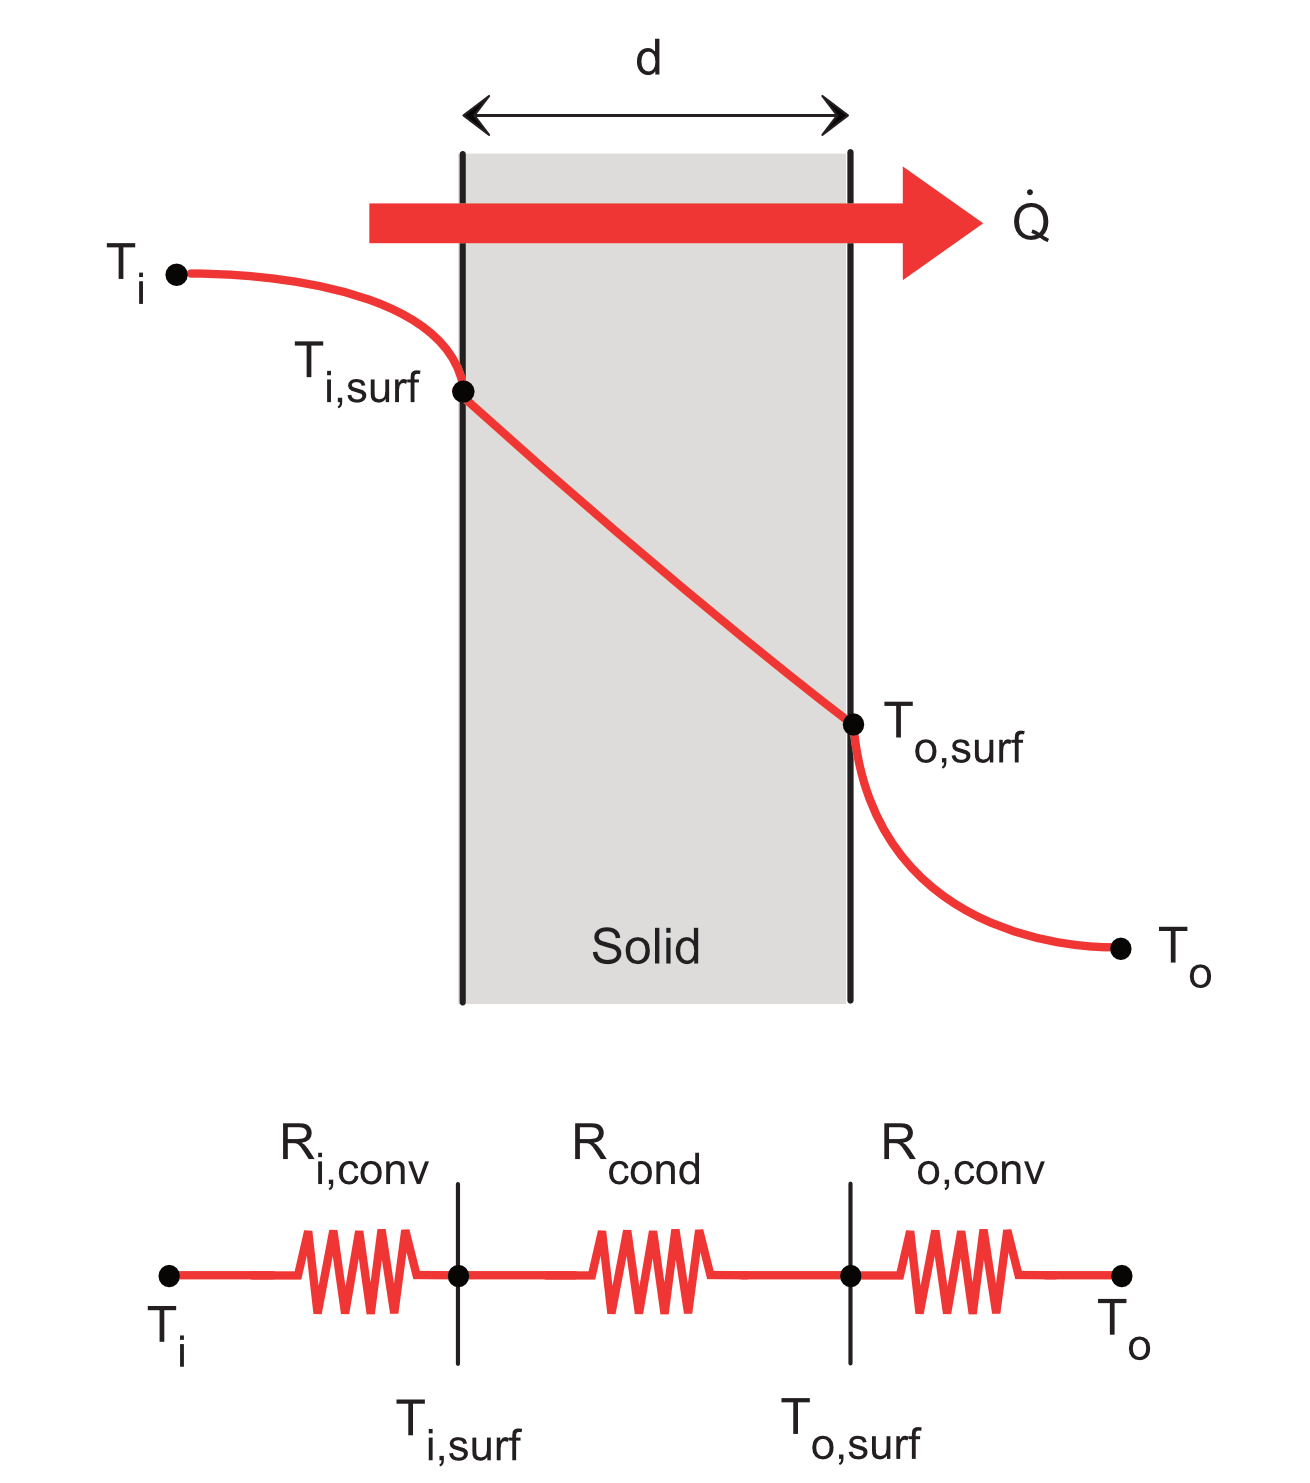
\includegraphics[scale=0.75]{Pictures/SimplePlate.png}
	\caption[SimplePlate]{The upper parts shows the side view sketch of a solid with a qualitative temperature profile (red line) and heat flow (red arrow). The lower part shows an analogous electrical circuit.}
	\label{fig:simpleplate}
\end{figure}

The total thermal resistance of the wall is a sum of the thermal resistance for convection at the inner surface, \(R_i^{conv}\), and outer surface, \(R_o^{conv}\), and on the thermal resistance of conduction: 
\begin{equation}
R_{tot} =  R_i^{conv} + R^{cond} + R_o^{conv}
\end{equation}
The thermal resistance for conduction, \(R^{cond}\), can be written as
\begin{equation}
R^{cond} =  \frac{d}{A}
\end{equation}
The thermal resistance for convection is usually expressed by the heat transfer coefficient $h^{conv}$, which is reciprocal to the thermal resistance
\begin{equation}
R^{conv} =  \frac{1}{h^{conv}}
\end{equation}
The resistance depends on the wind speed and wind direction and therefore depends on the overall geometry of the system. Their releationship is described in chapter \ref{chapter:windspeedrelation}.

Equation (1) has the form of Ohm's law. The thermal resistance corresponds to electrical resistance, temperature difference to voltage, and the heat transfer rate to electric current. Thus the problem can be solved by applying the thermal resistance concept in analogous manner to electrical circuit problems. The analogous electric circuit of the heating plate architecture is shown on the lower part of Fig. \ref{fig:simpleplate}. 


Fundamental knowledge on thermodnamics and on how to solve heat transfer problems can be found in the standard literature \cite{Cengel2002,Cengel2014}. 

\subsection{Heating Plate}\label{chapter:heatingplate}
In this chapter, the outer surface temperature of a heating plate in thermal equilibrium is derived. A picture of the architecture with such a heating plate buried in the midplane is shown in Fig. \ref{fig:platemodel}. \\

The outside ambient temperature is $T_o$ and the temperature in the inside of the sensor is $T_i$. Heat transfer takes place from the heated plate in the midplane to both the outside and to the inside of the front cover as illustrated by the red arrows in Fig. \ref{fig:platemodel}. 

\begin{figure} [H]
	\centering
	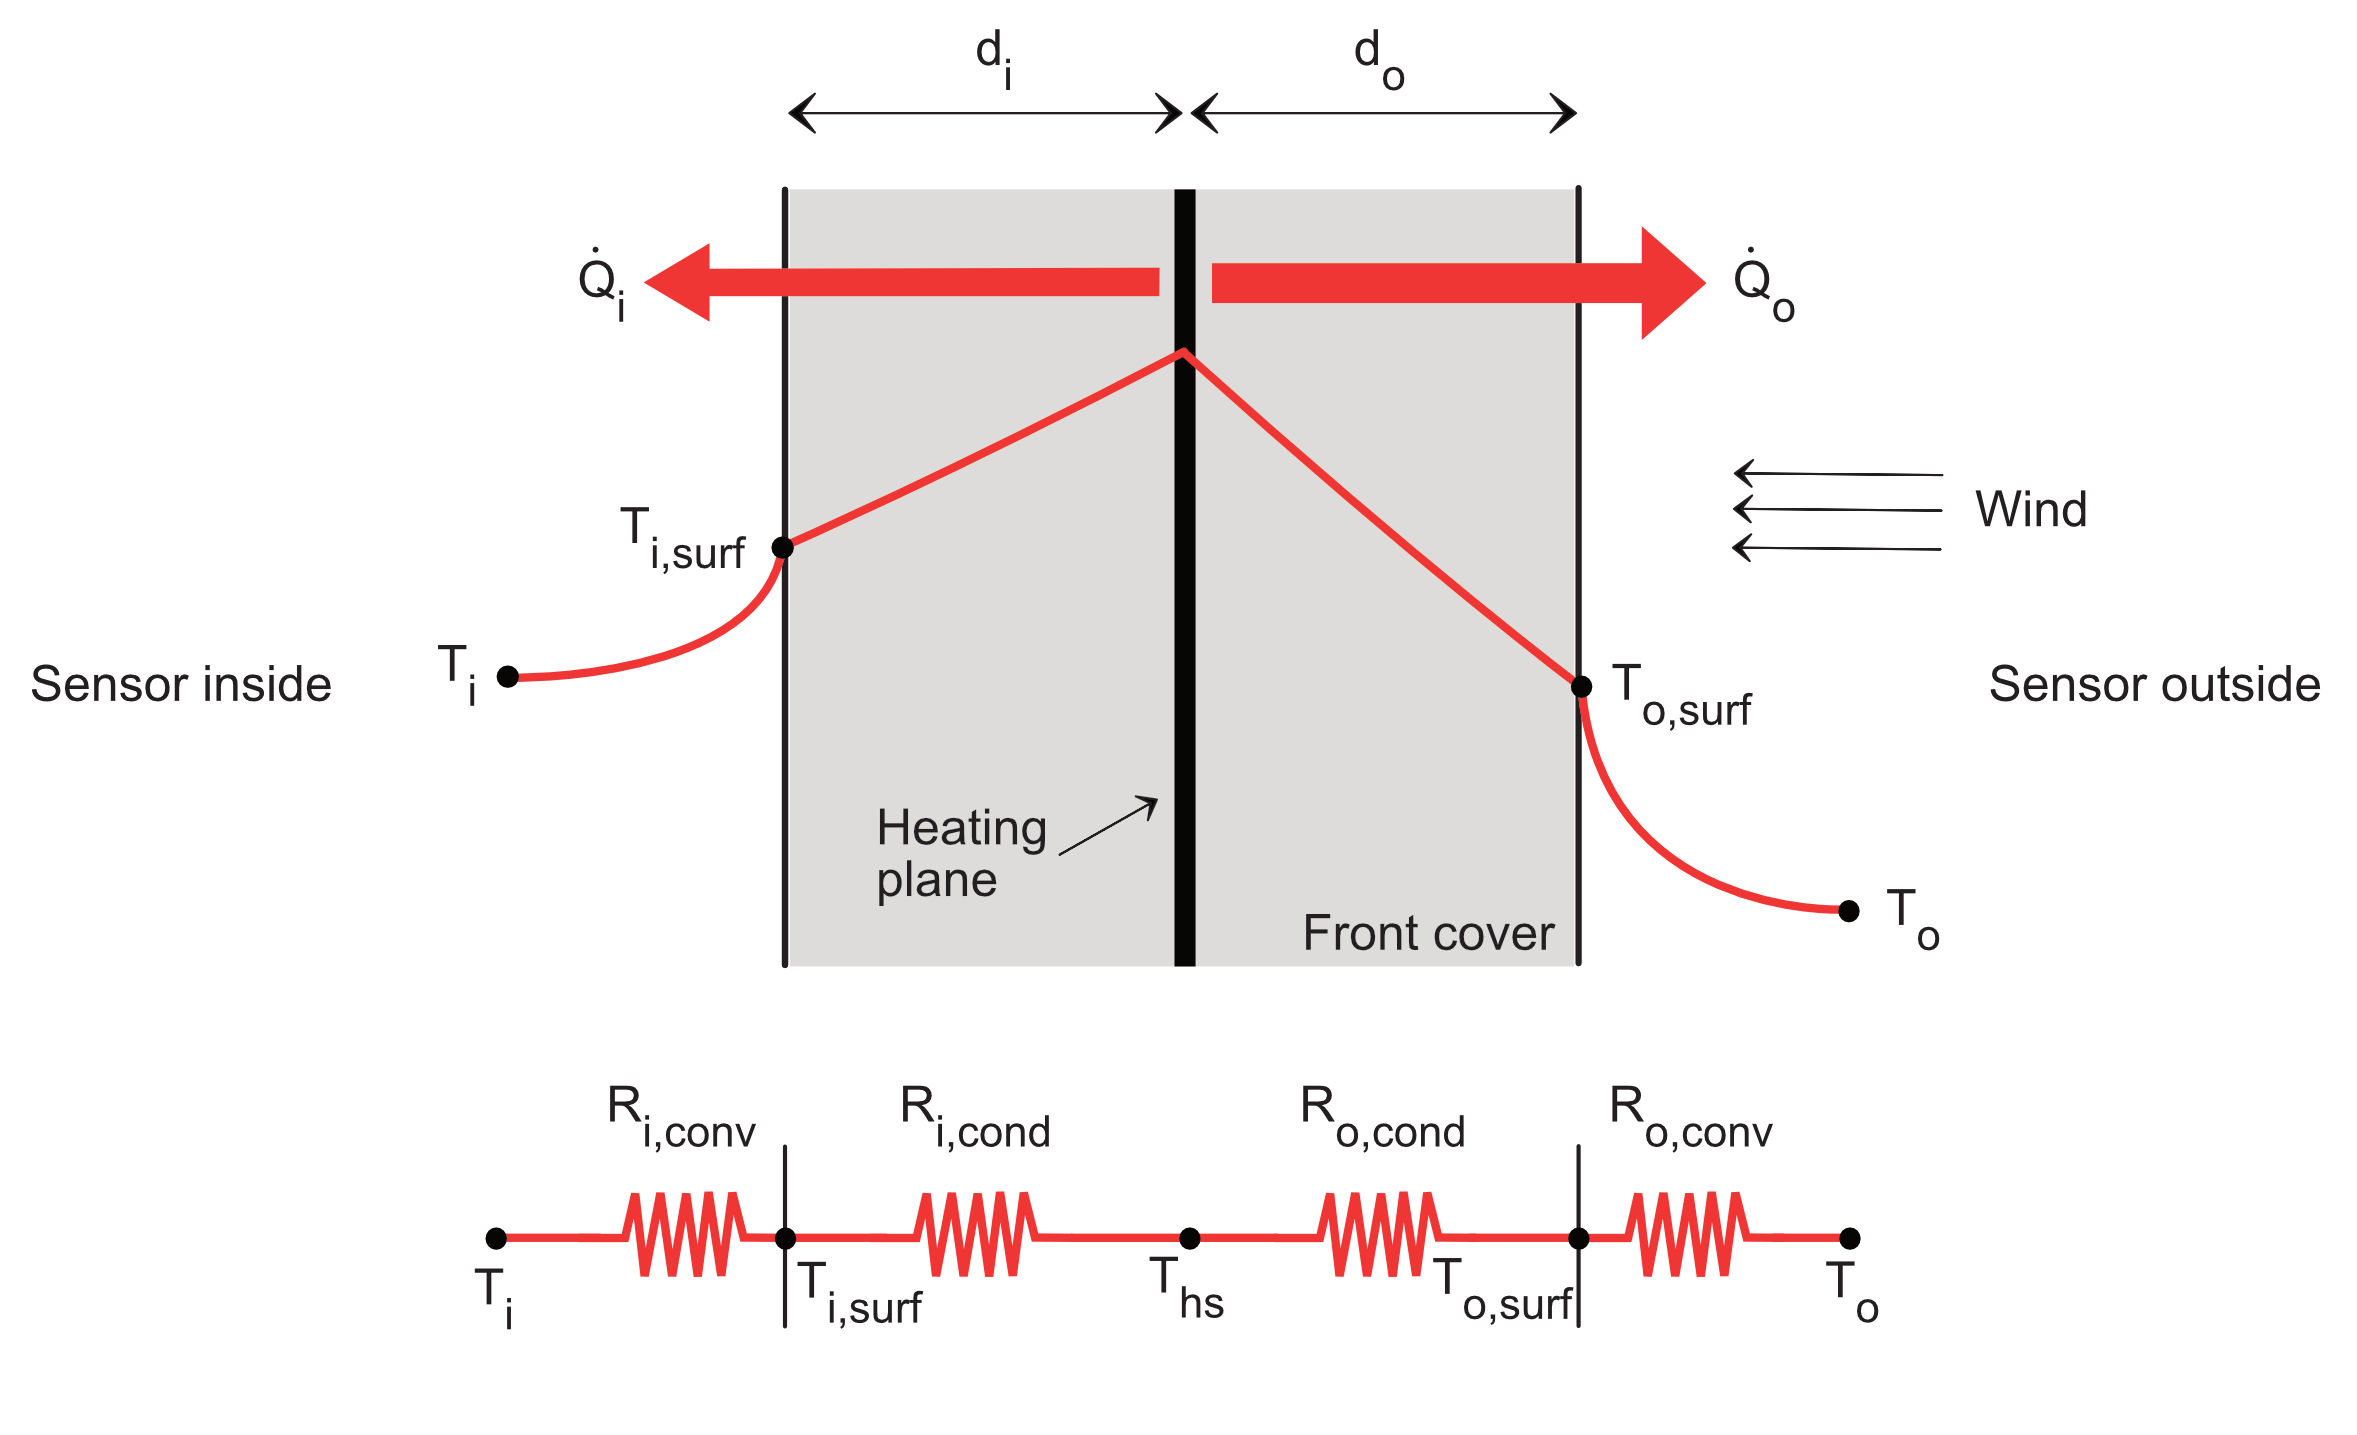
\includegraphics[scale=0.75]{Pictures/Model.png}
	\caption[Front Cover Heat Transfer Model]{Side view sketch of a front cover with a heating plate buried in the mid plane}
	\label{fig:platemodel}
\end{figure}
The outer surface temperature \(T_o^{surf}\) can be found by considering that the heat transfered in the system. The heat from the heating plate to the outer surface is transfered by conduction. Its heat rate is written as \(\dot Q_o^{cond}\). In thermal equilibrium, this heat rate is equal to the heat rate from the outer surface to the ambient, which is written as \(\dot Q_o^{conv}\):
\begin{equation}
\frac{\dot Q_o^{cond}}{A_h} = \frac{1}{R_o^{cond}}\cdot (T_{hs}-T_o^{surf}) \;\;\;\;\;\; = \;\;\;\;\;\;\frac{\dot Q_o^{conv}}{A_h} = \frac{1}{R_o^{conv}}\cdot (T_o^{surf}-T_{o})
\end{equation}
The conduction heat transfer rate per unit area \(\dot Q_{o,cond}/A_h\) is proportional to the temperature difference between the heating plate $T_{hs}$ and the outer surface \(T_o^{cond}\), where \(R_o^{cond}\) is the thermal resistance of the material expressed in \(m^2\cdot K/\mathrm{W}\). The thermal resistance for convection is usally defined as the inverse of the heat transfer coefficient \(R_o^{conv} = 1/h_o^{conv}\) expressed in \(\mathrm{W}/m^2\cdot K\). The surface temperature $T_o^{surf}$ can be derived by solving equation (1). It depends on the ambient temperature $T_o$ and the heating plate temperature $T_{hs}$:

(\(\dot Q_o^{conv}/A_h\)) 
(outer surface and the ambient)


\begin{eqnarray}
T_o^{surf} = T_o + \frac{R_o^{conv}}{R_{o}}\cdot(T_{hs}-T_o) \\
T_o^{surf} = \frac{R_o^{conv}}{R_{o}}\cdot T_{hs} + (1-\frac{R_o^{conv}}{R_{o}})\cdot T_o
\end{eqnarray}

To find the temperature of the heating plate $T_{hs}$ ($hs$ for heating source), the law of energy conservation is used. The total heat transfer rate per unit area \(\dot Q_{tot}/A_h\), or heating power \(P/A_h\) per unit area, is equal to the heat flux through the frontside \(\dot Q_o/A_h\) plus the heat flux through the backside \(\dot Q_i/A_h\) of the frontcover, where $A_h$ is the area through with the heat transfer takes place. 

The analogous electric circuit of the heating plate architecture is shown on the lower part of Fig. 2. 

\begin{equation}
\frac{P}{A} = \frac{\dot Q_o}{A_h} + \frac{\dot Q_i}{A_h} = \frac{1}{R_{i}}\cdot (T_{hs} - T_{i}) + \frac{1}{R_o}\cdot (T_{hs} - T_{o})
\end{equation}

Here, $R_i = R_i^{cond} + R_i^{conv}$ is the thermal resistance of unit area of the material between the heating plate and the sensor inside, which is equal to the sum of the conduction resistance and the convection resistance. Equally, $R_o = R_o^{cond} + R_o^{conv}$. Equation (1) can be expressed in another form
\begin{equation}
\frac{P}{A} = \frac{R_{tot}}{R_{o} R_{i}}\cdot(T_{hs}-T_{o}) - \frac{1}{R_{i}}\cdot(T_{i}-T_{o})
\end{equation}
The dissipated power per unit area ... Equation (4) consists of two terms: If the 
By rearranging equation (1), the temperature of the heating plate can be found to be 
\begin{equation}
T_{hs} = \frac{R_{o} R_{i}}{R_{tot}}\cdot\frac{P}{A} + \frac{R_{o}}{R_{tot}}\cdot(T_{i}-T_{o}) + T_{o} 
\end{equation}
with the total resistance of the front cover $R_{tot} = R_i + R_o$. Inserting $T_{hs}$ into equation (2) results in the expression for the surface temperature as a function of the heating power $P$, the ambient temperature $T_o$ and the heat transfer coefficient $h_o^{conv}$, which depends on the wind speed:
\begin{equation}
T_o^{surf} = T_o + \frac{R_o^{conv}}{R_o}\cdot(\frac{R_{o} R_{i}}{R_{tot}}\cdot\frac{P}{A} + \frac{R_{o}}{R_{tot}}\cdot(T_{i}-T_{o}))
\end{equation}
\begin{equation}
T_o^{surf} = T_o + \frac{R_o^{conv} R_{i}}{R_{tot}}\cdot\frac{P}{A} + \frac{R_o^{conv}}{R_{tot}}\cdot(T_{i}-T_{o})
\end{equation}
The surface temperature $T_o$ can be expressed as a function of the setpoint temperature, ambient temperature and the heating transfer coefficients:
\begin{eqnarray}
T_o^{surf} = a(R_o)\cdot T_{hs} + b(R_o)\cdot T_o \\
a(R_o) = \frac{R_o^{conv}}{R_o} \\
b(R_o) = 1-\frac{R_o^{conv}}{R_o}
\end{eqnarray}
%with $d_o$ the distance between the heating plate and the surface and $k$ the thermal conductivity of the material


%\begin{mdframed}[style=MyFrame]
%\begin{align}
%R_{tot} &=  R_{o}+ R_{i} \\
%R_{o} &=  R_o^{cond}+ R_o^{conv} \\
%R_{i} &=  R_i^{cond}+ R_i^{conv}
%\end{align}
%
%\end{mdframed}

\begin{figure}[ht]
\centering
\begin{minipage}[b]{0.48\linewidth}
\begin{figure} [H]
	\centering
	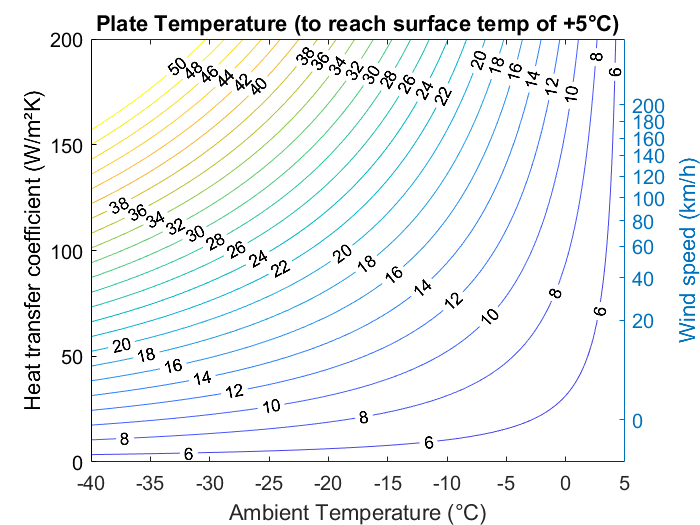
\includegraphics[scale=0.55]{Pictures/Plate_Tsurf5_PlateTemp.png}
	\caption[Heating Plate - Plate Temperature Graph]{Plate temperature (°C) required to reach an outer surface temperature of +5\dC.}
	\label{fig:PlateTemp}
\end{figure}

%\caption{Happy Smiley}
\label{fig:minipage1}
\end{minipage}
\quad
\begin{minipage}[b]{0.48\linewidth}
\begin{figure} [H]
	\centering
	\includegraphics[scale=0.55]{Pictures/Plate_Tsurf5_Power2.png}
	\caption[Heating Plate - Heating Power Graph]{Heating power (W) required to reach a outer surface temperature of +5\dC.}
	\label{fig:PlatePower}
\end{figure}
%\caption{Sad Smiley}
\label{fig:minipage2}
\end{minipage}
\end{figure}

\subsection{Relationship between Heat Transfer Coefficient and Wind Speed}\label{chapter:windspeedrelation}
The following table lists typical values of the heat transfer coefficient for different type of convection \cite{Cengel2002}: 




\begin{table} [H]
\centering
\color{B}
\begin{tabular} [h] {  p{50mm} p{27mm} }
Type of convection & $h, \unit{W/{m^2\cdot K}}$ \\ \hline
Natural convection of gases & 2 - 25 \\ 
Forced convection of gases & 10 - 250 
\end{tabular}
%\caption[Heat transfer coefficient of gases]{List of typical values for different heat transfer coefficients.}
%\label{tab:HTC}
\end{table}
The relationship between the heat transfer coefficient and the wind speed depends on the exact inflow and is therefore not easy to be calculated for the real system. The heat transfer coefficient for a low speed flow of air over a surface is about \(h_o^{conv} = 15 \,\,\,\unit{W/m^2\cdot K}\). Low speed means speeds below $1 \unit{km/h}$. This value gives well matching simulation results when comparing to experimental data recorded with the NEXT LiDAR sensor front cover. For higher wind speeds the following relation is the best fit to a series of data points shown in Fig. \ref{fig:HTC}: 
\begin{equation}
h_o^{conv} = h_0 + a\cdot \sqrt{v}
\end{equation}
with \(a = 25 \, \,\mathrm{W\cdot s^{1/2}/(K\cdot m^{5/2})}\) and the wind speed $v$ is given in m/s. 

\begin{figure} [H]
	\centering
	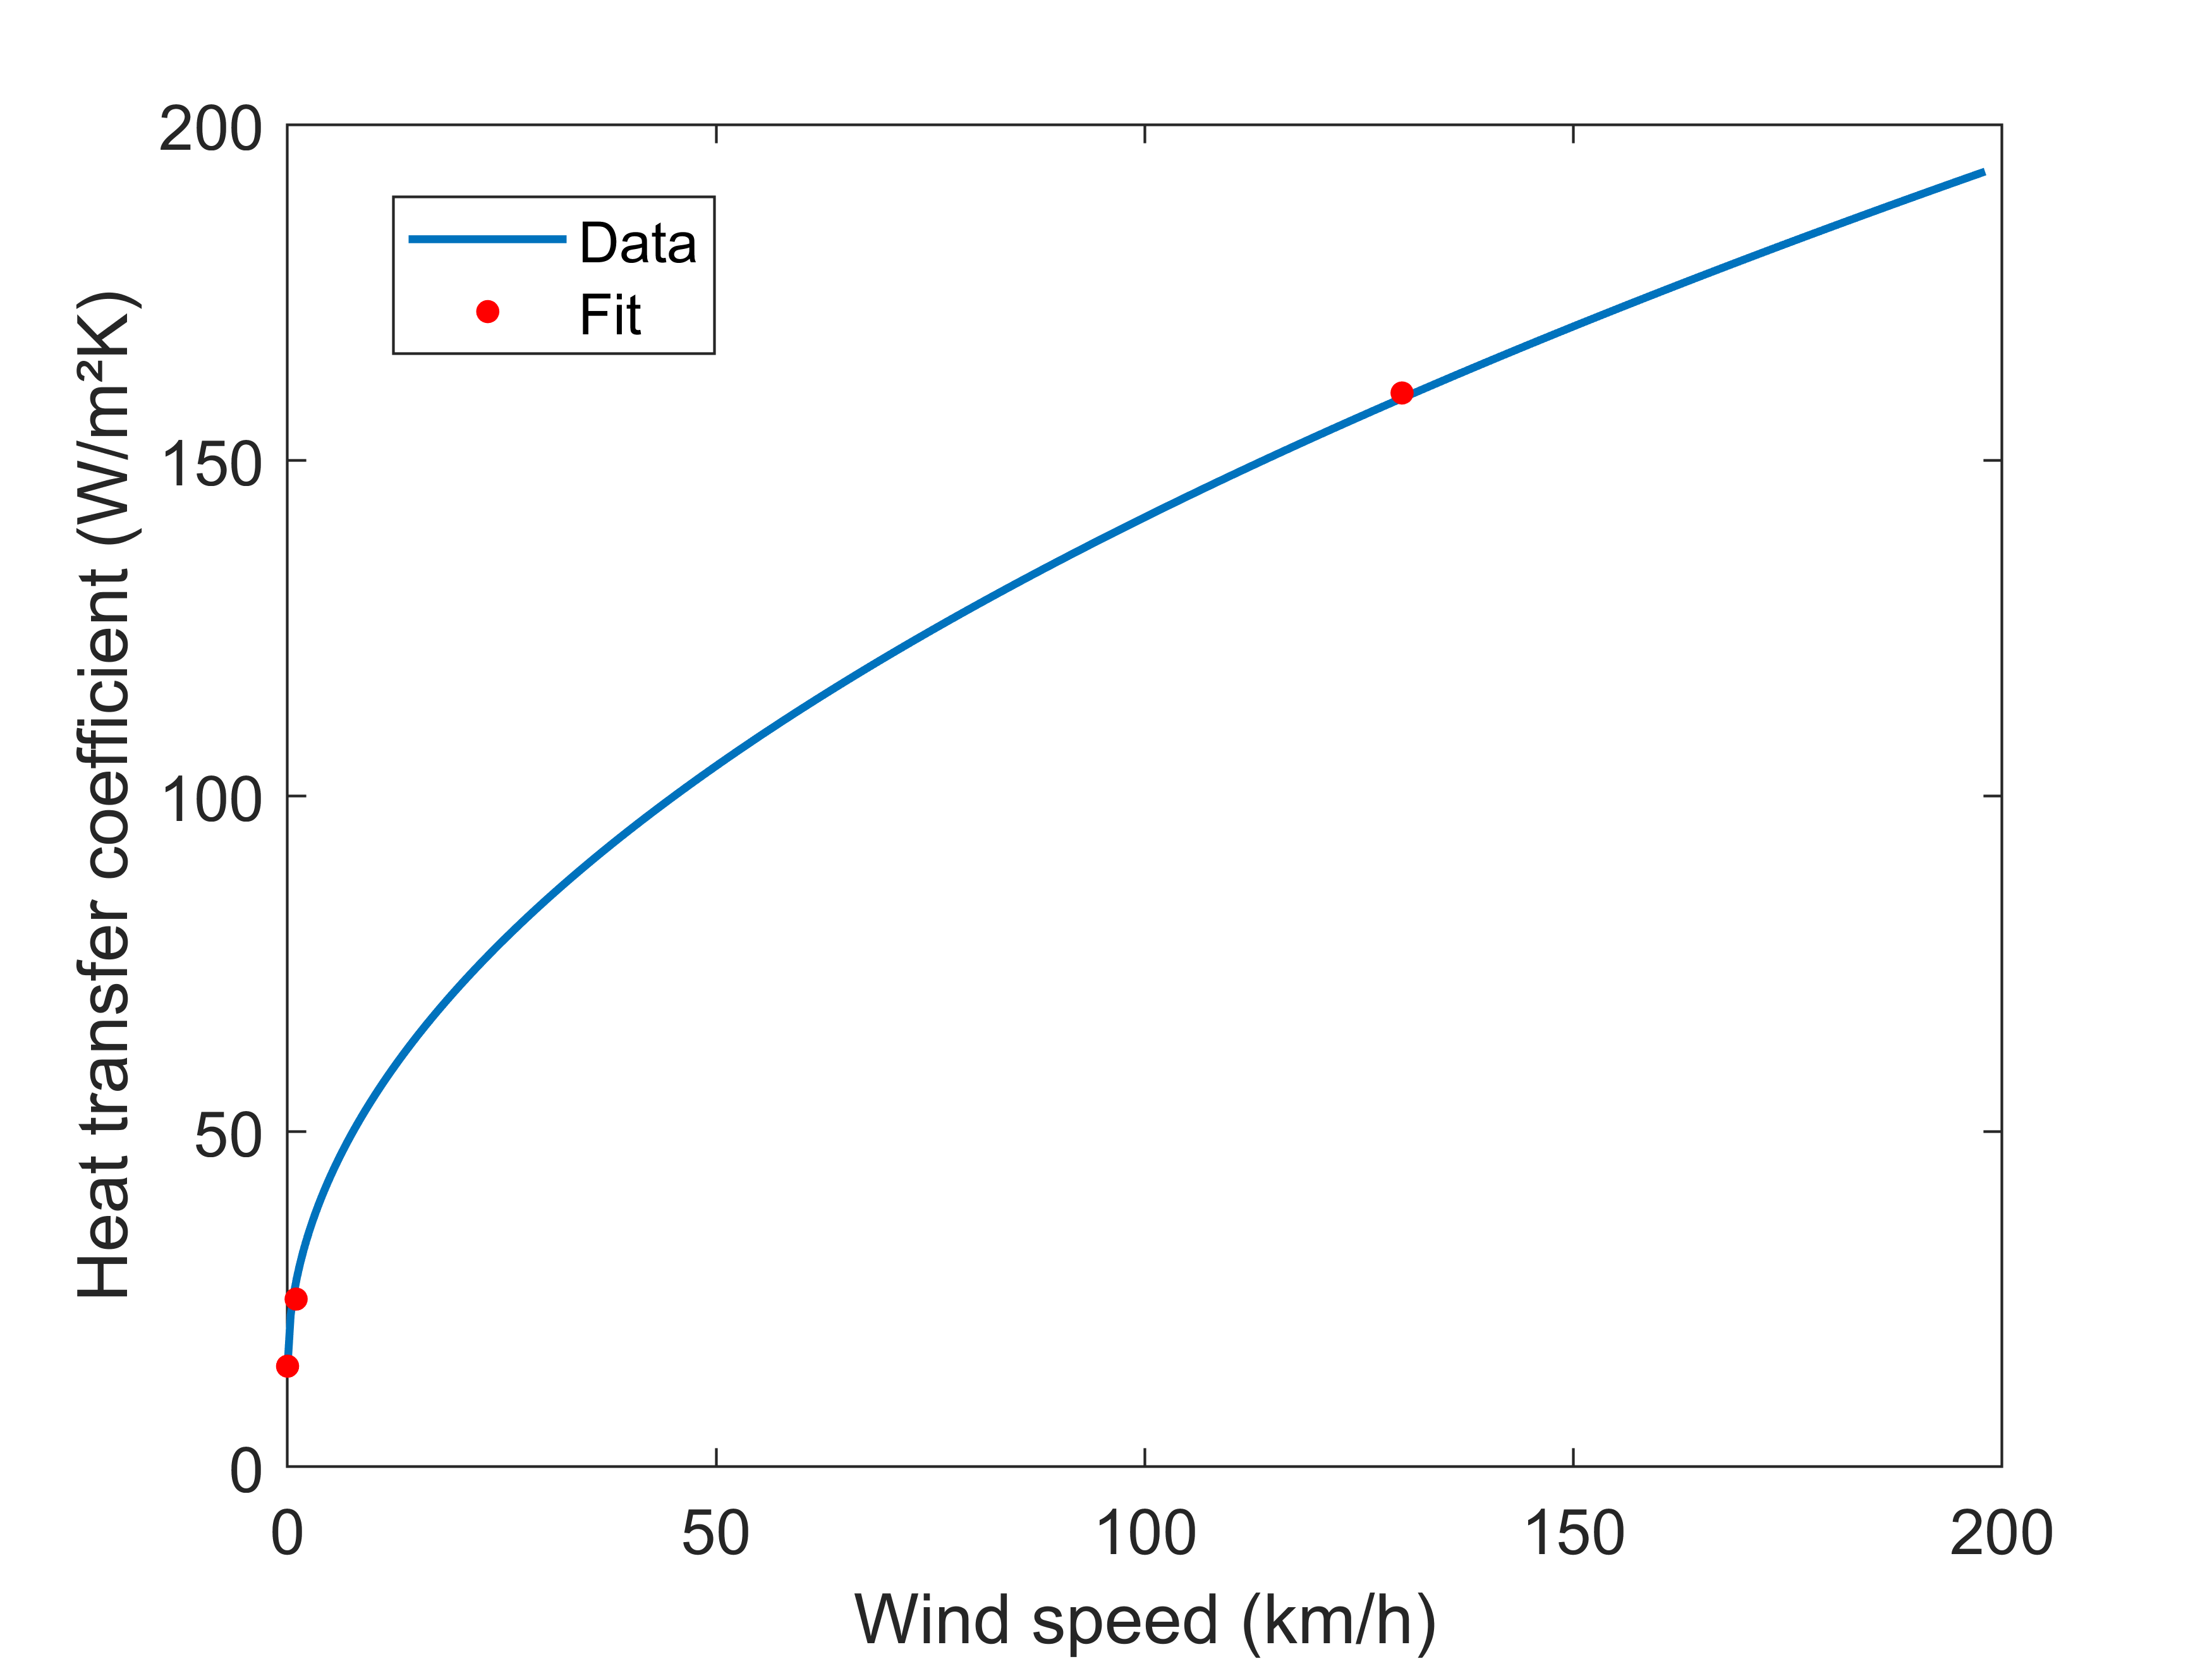
\includegraphics[scale=0.6]{Pictures/WindSpeed_Fit_Model2.png}
	\caption[Heat Transfer Coefficient vs Wind Speed]{Estimated heat transfer coefficient for the front cover outer surface of the NEXT 1T LiDAR sensor (in the B1 development phase) as a function of the wind speed. The plot shows the best fit (blue curve) to the series of data points from experiment and simulation (red dots).}
	\label{fig:HTC}
\end{figure}


%\begin{figure} [H]
%	\centering
%	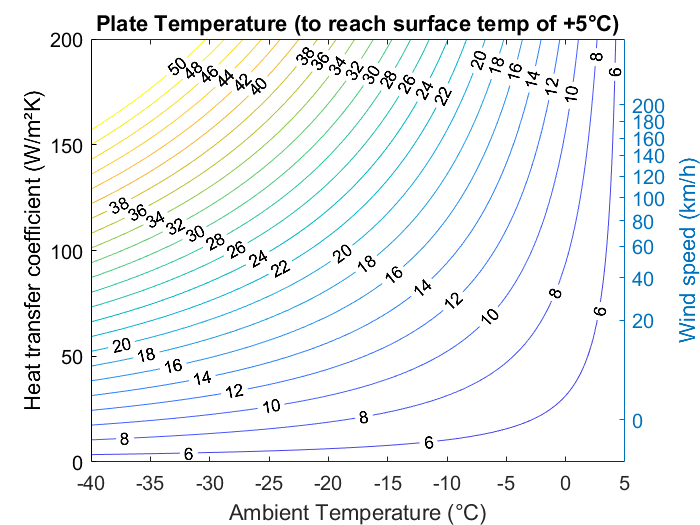
\includegraphics[scale=0.5]{Pictures/Plate_Tsurf5_PlateTemp.png}
%	\caption[Front Cover Heat Transfer Model]{Side view sketch of a front cover with a heating plate buried in the mid plane}
%	\label{fig:fig1}
%\end{figure}
%
%\begin{figure} [H]
%	\centering
%	\includegraphics[scale=0.5]{Pictures/Plate_Tsurf5_Power2.png}
%	\caption[Front Cover Heat Transfer Model]{Side view sketch of a front cover with a heating plate buried in the mid plane}
%	\label{fig:fig1}
%\end{figure}

\subsection{Heating Wire Architecture}
Shape Factor.\cite{Hahne1975}

\section{Front Cover Heating of the NEXT LiDAR Sensor}

\begin{figure} [H]
	\centering
	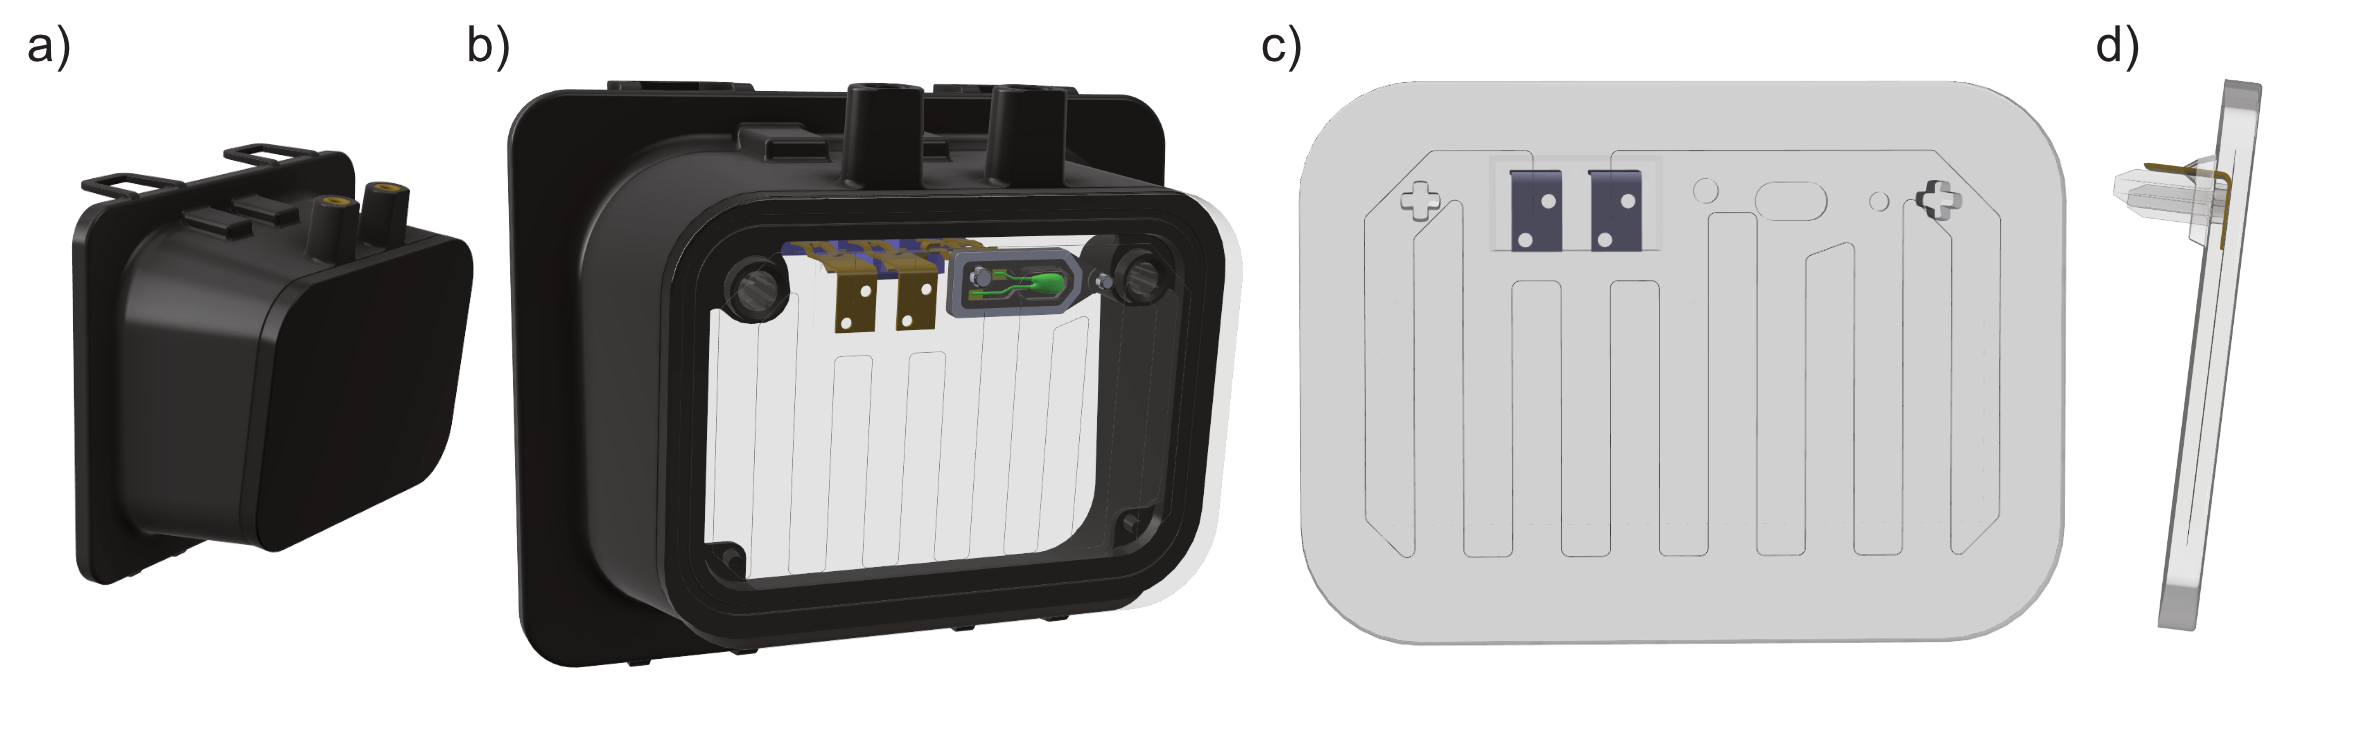
\includegraphics[scale=0.8]{Pictures/1TB1_3DModel.png}
	\caption[NEXT LiDAR Sensor Model]{ddd}
	\label{fig:1TB1Model}
\end{figure}


\begin{figure}[ht]
\centering
\begin{minipage}[b]{0.48\linewidth}
\begin{figure} [H]
	\centering
	\includegraphics[scale=0.55]{Pictures/1TB1_Tsurf5_WireTemp.png}
	\caption[Front Cover Heat Transfer Model]{Side view sketch of a front cover with a heating plate buried in the mid plane }
	\label{fig:fig1}
\end{figure}

%\caption{Happy Smiley}
\label{fig:minipage1}
\end{minipage}
\quad
\begin{minipage}[b]{0.48\linewidth}
\begin{figure} [H]
	\centering
	\includegraphics[scale=0.55]{Pictures/1TB1_Tsurf5_Power.png}
	\caption[Front Cover Heat Transfer Model]{Side view sketch of a front cover with a heating plate buried in the mid plane}
	\label{fig:fig1}
\end{figure}
%\caption{Sad Smiley}
\label{fig:minipage2}
\end{minipage}
\end{figure}


%TEXT
 

%\begin{table} [H]
%\color{B}
%\begin{tabular} [h] {p{30mm} | p{27mm} | p{27mm} | p{27mm} | p{27mm} }
%\rowcolor{LG}
% &  & & &  \\ \hlineRed
% &  &  &  & \\ \hline
% &  &  &  & \\
%\end{tabular}
%\caption[Name of an example table]{Name of an example table. Long text...}
%\label{tab:tab1}
%\end{table}

%\section{Key Performance Indicators}
%In this chapter, key figures are listed that should either be defined ....
